\documentclass{standalone}
\usepackage{graphicx}	
\usepackage{amssymb, amsmath}
\usepackage{color}

\usepackage{tikz}
\usetikzlibrary{intersections, backgrounds, math}
\usepackage{pgfmath}

\definecolor{light}{RGB}{220, 188, 188}
\definecolor{mid}{RGB}{185, 124, 124}
\definecolor{dark}{RGB}{143, 39, 39}
\definecolor{highlight}{RGB}{180, 31, 180}
\definecolor{light_teal}{RGB}{107, 142, 142}
\definecolor{mid_teal}{RGB}{72, 117, 117}
\definecolor{dark_teal}{RGB}{29, 79, 79}
\definecolor{gray10}{gray}{0.1}
\definecolor{gray20}{gray}{0.2}
\definecolor{gray30}{gray}{0.3}
\definecolor{gray40}{gray}{0.4}
\definecolor{gray60}{gray}{0.6}
\definecolor{gray70}{gray}{0.7}
\definecolor{gray80}{gray}{0.8}
\definecolor{gray90}{gray}{0.9}
\definecolor{gray95}{gray}{0.95}

\begin{document}

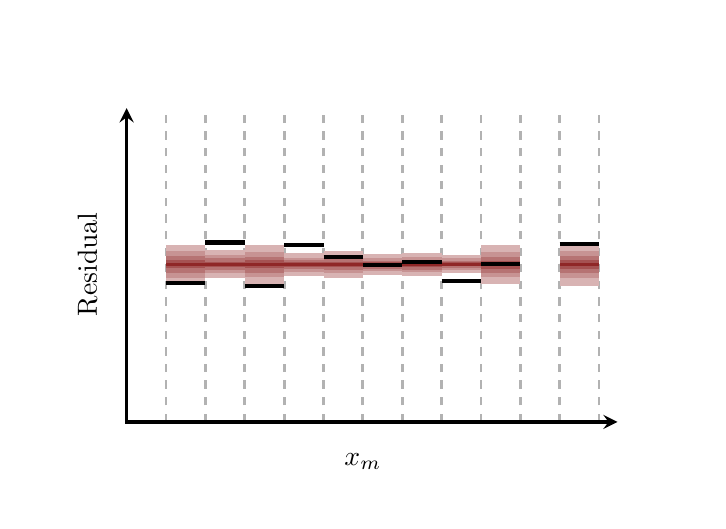
\begin{tikzpicture}[scale=1.0]
  
  \begin{scope}[shift={(8.5, 0)}]
    \draw[white] (-4.25, -3) rectangle (4.25, 3);
    
    \foreach \b in {-3.0, -2.5, ..., 3} {
      \draw[gray70, dashed, line width=1] (\b, -2) -- (\b, 2);
    }

    \pgfmathsetmacro{\ys}{0.4};
    \pgfmathsetmacro{\yo}{0};
    
    \pgfmathsetmacro{\prop}{20 + 15 * 1};
    \colorlet{custom}{dark!\prop!white};
    
    \foreach \a/\b/\c/\d  in {-2.500/-2.000/-0.663/0.619, -2.000/-1.500/-0.417/0.445, -1.500/-1.000/-0.624/0.604, -1.000/-0.500/-0.370/0.353, -0.500/0.000/-0.422/0.429, 0.000/0.500/-0.329/0.334, 0.500/1.000/-0.373/0.368, 1.000/1.500/-0.273/0.304, 1.500/2.000/-0.633/0.618, 2.500/3.000/-0.674/0.647} {
       \fill[custom] (\a, \ys * \c + \yo) rectangle (\b, \ys * \d + \yo);
    }
    
    \pgfmathsetmacro{\prop}{20 + 15 * 2};
    \colorlet{custom}{dark!\prop!white};
    
    \foreach \a/\b/\c/\d  in {-2.500/-2.000/-0.433/0.424, -2.000/-1.500/-0.271/0.289, -1.500/-1.000/-0.409/0.397, -1.000/-0.500/-0.239/0.218, -0.500/0.000/-0.273/0.271, 0.000/0.500/-0.204/0.211, 0.500/1.000/-0.247/0.249, 1.000/1.500/-0.171/0.211, 1.500/2.000/-0.410/0.403, 2.500/3.000/-0.429/0.415, } {
       \fill[custom] (\a, \ys * \c + \yo) rectangle (\b, \ys * \d + \yo);
    }
    
    \pgfmathsetmacro{\prop}{20 + 15 * 3};
    \colorlet{custom}{dark!\prop!white};
    
    \foreach \a/\b/\c/\d  in {-2.500/-2.000/-0.272/0.261, -2.000/-1.500/-0.166/0.192, -1.500/-1.000/-0.256/0.246, -1.000/-0.500/-0.152/0.140, -0.500/0.000/-0.170/0.173, 0.000/0.500/-0.134/0.125, 0.500/1.000/-0.163/0.157, 1.000/1.500/-0.109/0.118, 1.500/2.000/-0.263/0.249, 2.500/3.000/-0.282/0.269} {
       \fill[custom] (\a, \ys * \c + \yo) rectangle (\b, \ys * \d + \yo);
    }
    
    \pgfmathsetmacro{\prop}{20 + 15 * 4};
    \colorlet{custom}{dark!\prop!white};
    
    \foreach \a/\b/\c/\d  in {-2.500/-2.000/-0.115/0.127, -2.000/-1.500/-0.076/0.089, -1.500/-1.000/-0.120/0.128, -1.000/-0.500/-0.071/0.065, -0.500/0.000/-0.080/0.077, 0.000/0.500/-0.067/0.063, 0.500/1.000/-0.081/0.076, 1.000/1.500/-0.059/0.064, 1.500/2.000/-0.131/0.124, 2.500/3.000/-0.143/0.141,} {
       \fill[custom] (\a, \ys * \c + \yo) rectangle (\b, \ys * \d + \yo);
    }
    
     \foreach \a/\b/\c  in {-2.500/-2.000/0.000, -2.000/-1.500/0.000, -1.500/-1.000/0.000, -1.000/-0.500/0.000, -0.500/0.000/0.000, 0.000/0.500/0.000, 0.500/1.000/0.000, 1.000/1.500/0.000, 1.500/2.000/0.000,2.500/3.000/0.000} {
       \draw[dark, line width=1] (\a, \ys * \c + \yo) -- (\b, \ys * \c + \yo);
    }
    
    
    \foreach \l/\r/\m in {-2.500/-2.000/-0.581, -2.000/-1.500/0.695, -1.500/-1.000/-0.685, -1.000/-0.500/0.619, -0.500/0.000/0.241, 0.000/0.500/-0.018, 0.500/1.000/0.074, 1.000/1.500/-0.515, 1.500/2.000/0.022, 2.500/3.000/0.654} {
      \draw[black, line width=1.5] (\l, \ys * \m + \yo) -- (\r, \ys * \m + \yo);
    }
     
    \draw [->, >=stealth, line width=1.25] (-3.00, -2.015) -- +(0, 4);
    \draw [->, >=stealth, line width=1.25] (-3.015, -2.00) -- +(6.25, 0);
    
    \node[rotate=90] at (-3.5, 0) { Residual };
    \node at (0, -2.5) { $x_{m}$ };
  \end{scope}
  
\end{tikzpicture}

\end{document}  